\documentclass[11pt]{article}

\usepackage[margin=1in]{geometry}
\usepackage{graphicx}
\usepackage{booktabs}
\usepackage{amsmath}
\usepackage{amssymb}
\usepackage{authblk}
\usepackage{hyperref}
\usepackage[numbers,sort&compress]{natbib}
\usepackage{caption}
\usepackage{subcaption}
\usepackage{float}
\usepackage{xcolor}
\usepackage{xurl}

\hypersetup{
  colorlinks=true,
  linkcolor=blue,
  citecolor=blue,
  urlcolor=blue
}

\title{\textbf{Latent predictive pretraining improves a conservative neural force field on molecular dynamics trajectories}}
\author{Tanmay Sarkar Akash$^{1}$ and Siddhartha Das$^{1,*}$}
\affil{$^{1}$Department of Mechanical Engineering, University of Maryland, College Park, MD 20742\\
$^{*}$Email: \texttt{sidd@umd.edu}}
\date{}

\begin{document}
\maketitle

\noindent\textbf{Machine-learning force fields (MLFFs) can approach quantum-mechanical-level accuracy at a computational cost closer to classical force fields, but they remain constrained by the expense of labelled energy and force data. Here we test whether joint-embedding predictive architecture (JEPA) pretraining, adapted to atomistic trajectories, can improve a conservative neural molecular force field. We used the ethanol trajectory from the MD17 benchmark, pretrained a SchNet-like continuous-filter encoder to predict latent embeddings of masked atomic environments at neighbouring time steps, then fine-tuned the same encoder to predict molecular energies and forces. In a 2,000/500/500 train/validation/test split trained for 50 epochs, JEPA initialization reduced test force RMSE from 1.963 to 1.666 in native MD17 force units and reduced energy MAE from 4.266 to 1.058 in native MD17 energy units relative to a scratch baseline. These preliminary results suggest that latent predictive pretraining can transfer useful dynamical structure from unlabelled molecular trajectories into supervised neural force-field learning.}

\section*{}

Molecular dynamics (MD) requires force fields that provides a potential energy surface with its gradients produce physically meaningful forces. Classical force fields provide speed but can lack electronic accuracy, whereas direct \textit{ab initio} MD is often too expensive for long trajectories or large systems. Machine-learning interatomic potentials have emerged as a compromise: they learn quantum-mechanical energy and force labels while retaining efficient evaluation in simulation. Gradient-domain force-field methods and the MD17 benchmark, continuous-filter neural networks and modern equivariant graph neural networks have established that molecular symmetries and conservative force construction are central to accuracy and data efficiency~\cite{chmiela2017gdml, chmiela2018exact, schutt2017schnet, batzner2022nequip, batatia2022mace, musaelian2023allegro}.

Inherently, neural force-field training needs to be predominantly supervised. This is restrictive because high-quality quantum-mechanical energy and force labels require expensive electronic-structure calculations, whereas molecular geometries and trajectories from classical force fields, lower-level simulations or existing archives are easier to collect at scale. Self-supervised learning offers a possible route around this bottleneck by learning from coordinates before using scarce high-level labels. In our experiment below, the pretraining stage deliberately treats the available trajectory coordinates as unlabelled and ignores the accompanying energies and forces until fine-tuning. In vision, joint-embedding predictive architectures learn representations by predicting latent target embeddings from partial context rather than reconstructing raw pixels~\cite{assran2023ijepa}. An analogous principle is appealing for molecules: atomic coordinates are continuous, noisy, symmetry-constrained and often locally ambiguous, but latent neighbourhood representations may capture stable dynamical regularities.

Here we implemented an atomistic JEPA pretraining workflow for a small-molecule neural force field. The model uses a compact SchNet-like continuous-filter encoder over atomic numbers and pairwise distances. The energy is invariant to rigid translations and rotations, and forces are obtained as negative coordinate gradients of the scalar energy, making the learned force field conservative and force predictions equivariant under rigid rotations. During pretraining, an online encoder receives a corrupted molecular frame in which a random subset of atoms is replaced by a learned mask token. An exponential-moving-average target encoder receives the uncorrupted frame at the next trajectory step. A predictor network is trained to match the target latent embeddings on masked atoms. The pretrained encoder is then fine-tuned using energy and force labels.

\subsection*{Mathematical formulation}

We represent an MD trajectory as a sequence of atomistic states
\begin{equation}
    x_t = (Z, R_t, E_t, F_t),
\end{equation}
where $Z \in \mathbb{N}^{N}$ are atomic numbers for $N$ atoms, $R_t \in \mathbb{R}^{N \times 3}$ are Cartesian coordinates, $E_t \in \mathbb{R}$ is the reference potential energy and $F_t \in \mathbb{R}^{N \times 3}$ are reference forces. The encoder $f_{\theta}$ maps atomic numbers and coordinates to atomwise latent embeddings,
\begin{equation}
    H_t = f_{\theta}(Z, R_t) \in \mathbb{R}^{N \times d}.
\end{equation}

For JEPA pretraining, we sample a binary atom mask $m \in \{0,1\}^{N}$, where $m_i=1$ indicates that atom $i$ is hidden from the context branch. The online encoder receives a corrupted context frame $\tilde{x}_t=(Z,\tilde{R}_t,m)$, implemented by replacing masked atom embeddings with a learned mask token, while the target encoder receives a clean future frame $x_{t+\Delta}$. With online encoder $f_{\theta}$, target encoder $f_{\bar{\theta}}$, predictor $q_{\phi}$ and stop-gradient operator $\operatorname{sg}(\cdot)$, the pretraining loss is
\begin{equation}
\mathcal{L}_{\mathrm{JEPA}}(\theta,\phi)
=
\frac{1}{\sum_i m_i}
\sum_{i=1}^{N}
m_i
\left\|
q_{\phi}\!\left(f_{\theta}(Z,\tilde{R}_t,m)_i\right)
-
\operatorname{sg}\!\left(f_{\bar{\theta}}(Z,R_{t+\Delta})_i\right)
\right\|_2^2 .
\label{eq:jepa}
\end{equation}

The target parameters are not optimized by backpropagation. Instead, they follow the online encoder through an exponential moving average,
\begin{equation}
    \bar{\theta} \leftarrow \tau \bar{\theta} + (1-\tau)\theta,
\end{equation}
with $\tau=0.99$ in our experiments. After pretraining, the online encoder initializes the supervised force-field model.

The supervised model predicts a scalar potential energy as a sum of atomwise contributions,
\begin{equation}
    \hat{E}_{\psi}(Z,R)
    =
    b_E
    +
    \sum_{i=1}^{N}
    g_{\psi}\!\left(f_{\theta}(Z,R)_i\right),
    \label{eq:energy}
\end{equation}
where $g_{\psi}$ is an energy head and $b_E$ is the train-set mean energy offset. Predicted forces are conservative by construction:
\begin{equation}
    \hat{F}_{\psi}(Z,R)
    =
    -\nabla_R \hat{E}_{\psi}(Z,R).
    \label{eq:forces}
\end{equation}

Fine-tuning minimizes a force-dominant supervised objective,
\begin{equation}
    \mathcal{L}_{\mathrm{sup}}
    =
    \lambda_E
    \left\|
    \hat{E}_{\psi} - E
    \right\|_1
    +
    \lambda_F
    \left\|
    \hat{F}_{\psi} - F
    \right\|_2^2 ,
    \label{eq:supervised}
\end{equation}
with $\lambda_E=0.05$ and $\lambda_F=1.0$. Evaluation reports energy MAE, force MAE and force RMSE on the held-out test trajectory frames.

We evaluated the workflow on ethanol from MD17, a standard DFT molecular dynamics benchmark containing atomic numbers, coordinates, energies and forces. The experiment used 2,000 frames for training, 500 for validation and 500 for testing. Both scratch and JEPA-initialized force fields were trained for 50 epochs with identical supervised hyperparameters. The scratch baseline reached a best validation force RMSE of 1.596 and a final test force RMSE of 1.963. The JEPA-initialized model reached a best validation force RMSE of 1.322 and a final test force RMSE of 1.666. On the test set, JEPA pretraining improved force RMSE by 15.2\%, force MAE by 12.6\% and energy MAE by 75.2\% relative to the scratch baseline (Table~\ref{tab:results}).

To separate representation learning from supervised force-field fitting, we tracked both the JEPA pretraining objective and downstream validation force error (Fig.~\ref{fig:summary}). The self-supervised JEPA objective improved quickly: validation loss reached its minimum at epoch 9 (0.00119), before the end of the 50-epoch pretraining run. Downstream fine-tuning continued to improve force accuracy over the full supervised training run. This suggests that early stopping or a validation-selected JEPA checkpoint should be included in larger studies, although the final JEPA checkpoint still transferred effectively to supervised force-field training in this single-molecule experiment.

These results should be interpreted as a proof of concept rather than a benchmark claim. The encoder is intentionally lightweight and uses invariant scalar message passing rather than full tensor-equivariant interactions. The split is chronological and limited to one molecule, one random seed and one dataset size. The reported units are the native units stored in the downloaded MD17 \texttt{.npz} file and are not converted to the units used in all published rMD17 leaderboards. Even with these limitations, the controlled scratch-versus-pretrained comparison supports the central hypothesis: latent prediction over MD trajectories can provide useful initialization for conservative neural force fields.

The self-supervised JEPA objective improved quickly: validation loss reached its minimum at epoch 9 (0.00119), before the end of the 50-epoch pretraining run. In the verified route, both pretraining and fine-tuning use the same DFT trajectory distribution, but pretraining treats the coordinates as unlabelled and withholds the accompanying energies and forces. The improvement over a randomly initialized force field therefore demonstrates that a DFT-coordinate-only self-supervised stage can improve subsequent supervised DFT force-field learning in this ethanol setting. A second route is cross-fidelity pretraining, in which JEPA first learns from larger pools of classical, semiempirical or mixed-fidelity trajectories and is then fine-tuned only on high-level DFT labels. This route is attractive because lower-cost trajectories are easier to generate at scale, but it remains unverified in the present work and may help only when their coordinate distribution overlaps the target quantum-mechanical distribution.

Future work should test whether the effect persists across all rMD17 molecules, multiple random seeds, smaller labelled-data regimes and true tensor-equivariant backbones such as NequIP or MACE. The most important next experiment is label-efficiency: if JEPA pretraining provides larger gains when only tens to hundreds of labelled DFT frames are available, it would directly address the data bottleneck that limits practical ML force-field construction.

\begin{table}[H]
\centering
\caption{\textbf{Test performance after 50 supervised epochs.} Metrics are reported in the native units of the downloaded MD17 ethanol \texttt{.npz} file. The drift proxy is the mean absolute force error and is included as a simple local surrogate for force-driven rollout error.}
\label{tab:results}
\begin{tabular}{lrrrr}
\toprule
Model & Energy MAE & Force MAE & Force RMSE & Drift proxy \\
\midrule
Scratch & 4.266 & 1.458 & 1.963 & 1.458 \\
JEPA initialized & 1.058 & 1.274 & 1.666 & 1.274 \\
Relative improvement & 75.2\% & 12.6\% & 15.2\% & 12.6\% \\
\bottomrule
\end{tabular}
\end{table}

\begin{figure}[H]
\centering
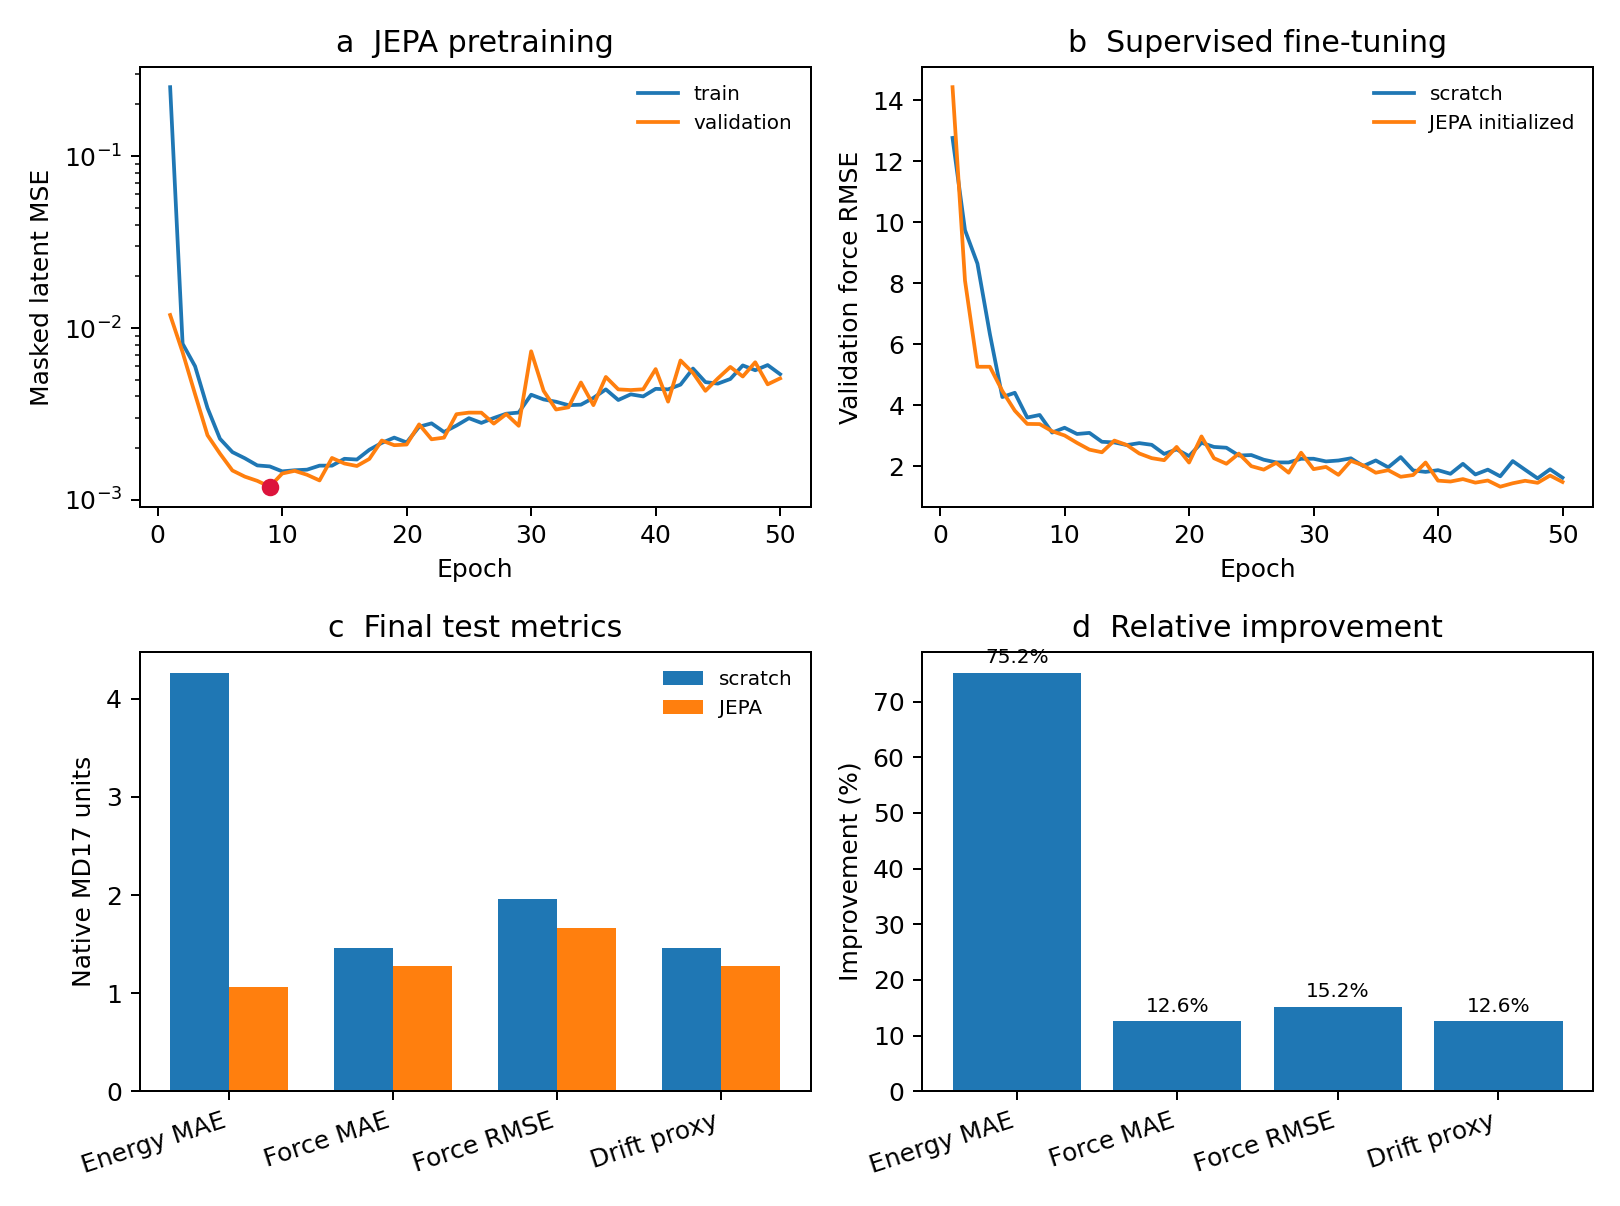
\includegraphics[width=\linewidth]{../results/summary_panel_50.png}
\caption{\textbf{Training dynamics and test performance.} (a) JEPA pretraining loss for masked latent prediction. The validation loss reaches its minimum at epoch 9. (b) Validation force RMSE during supervised fine-tuning for scratch and JEPA-initialized models. (c) Final test metrics on the held-out MD17 ethanol split. (d) Relative improvement of JEPA initialization over scratch training.}
\label{fig:summary}
\end{figure}

\begin{figure}[H]
\centering
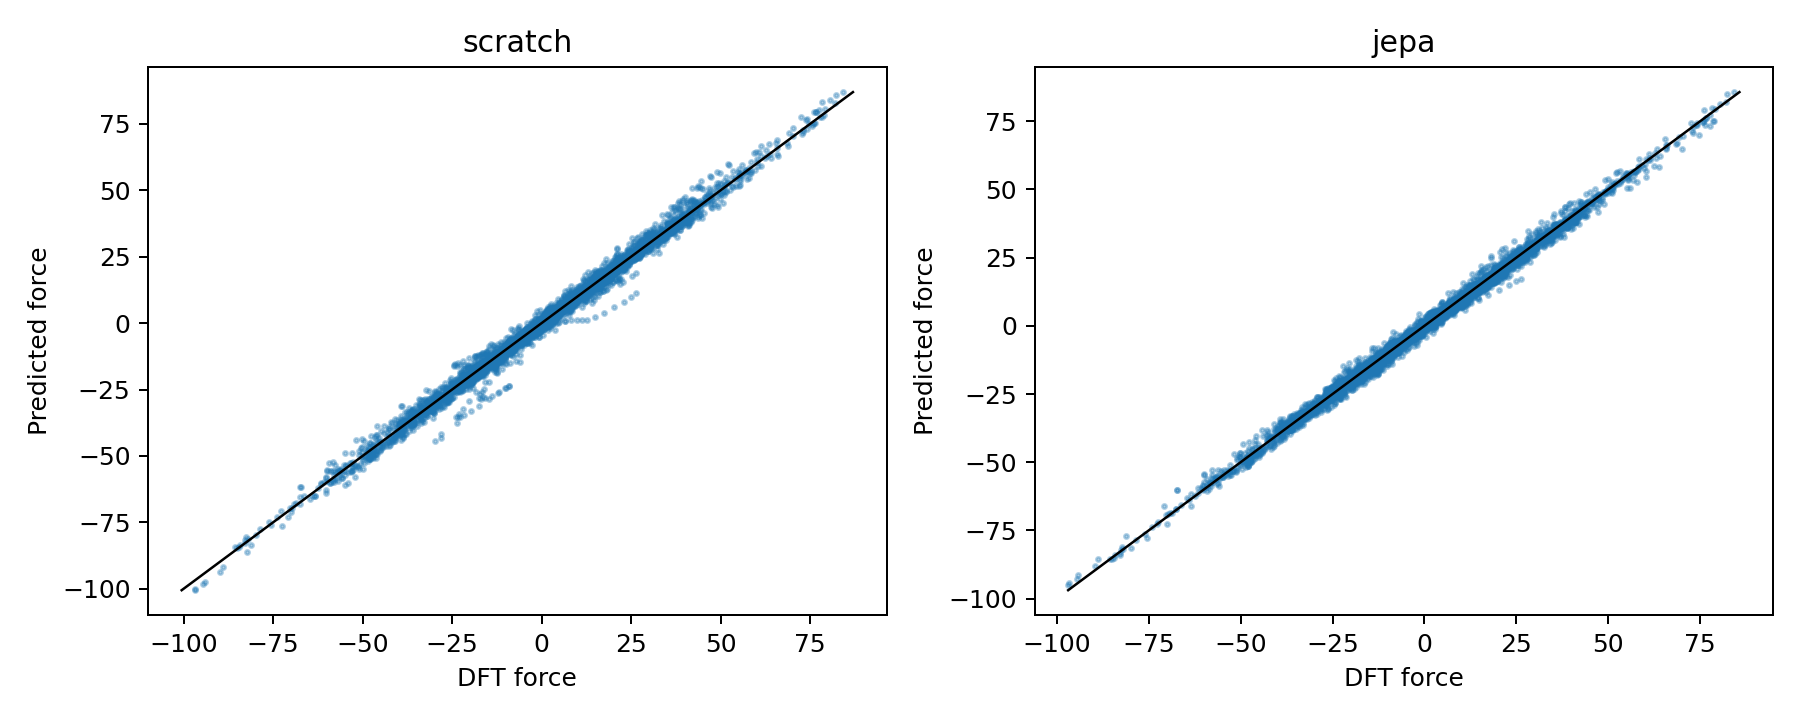
\includegraphics[width=0.95\linewidth]{../results/force_scatter_50.png}
\caption{\textbf{Force prediction scatter for scratch and JEPA-initialized models.} Predicted force components are plotted against DFT reference force components for the held-out MD17 ethanol test split. The diagonal line indicates perfect agreement. The JEPA-initialized model exhibits a lower force RMSE than the scratch baseline after the same number of supervised epochs.}
\label{fig:force_scatter}
\end{figure}

\section*{Methods}

\subsection*{Dataset}
The ethanol trajectory was downloaded from the canonical sGDML/MD17 data endpoint using \texttt{scripts/download\_md17.py}. MD17 was introduced for learning energy-conserving molecular force fields from \textit{ab initio} molecular dynamics trajectories, and the revised MD17 literature motivates careful treatment of energy and force labels in molecular force-field benchmarks~\cite{chmiela2017gdml, christensen2020gradients}. The validated file contained 555,092 frames and 9 atoms with atomic numbers $[6,6,8,1,1,1,1,1,1]$. Arrays were normalized to the internal key convention \texttt{z}, \texttt{R}, \texttt{E} and \texttt{F}. The experiment used the first 2,000 frames for training, the next 500 for validation and the next 500 for testing.

\subsection*{Model}
The encoder is a compact SchNet-like network with atom embeddings, Gaussian radial basis distance features, continuous-filter message passing and layer normalization. The force-field head predicts atomic energy contributions that are summed into a molecular energy. A train-set mean energy offset is stored as a non-trainable buffer. Forces are calculated by automatic differentiation as $F=-\mathrm{d}E/\mathrm{d}R$, ensuring a conservative force field.

\subsection*{JEPA pretraining}
The JEPA stage uses an online encoder, an EMA target encoder and a predictor MLP. For each molecular frame, a random subset of atoms is masked in the online branch. The target branch receives the uncorrupted frame at temporal offset $\Delta=1$. The training loss is masked latent mean-squared error between predictor outputs and stop-gradient target embeddings. The default mask ratio is 0.35 and EMA decay is 0.99. The 50-epoch pretraining checkpoint is \path{checkpoints/jepa_pretrained_50.pt}.

\subsection*{Supervised fine-tuning}
Scratch and JEPA-initialized force fields were trained with the same supervised objective in Eq.~\ref{eq:supervised}. Both models were trained for 50 epochs using AdamW. The scratch model was initialized randomly. The JEPA model loaded the pretrained encoder weights and initialized a fresh energy head.

\subsection*{Evaluation}
Evaluation was performed on the held-out 500-frame test set. Metrics were energy MAE, force MAE and force RMSE. A simple drift proxy was defined as mean absolute force error. This proxy is not a substitute for long-time MD rollout validation, but captures local force error relevant to short-step integration.

\section*{Data availability}
The MD17 ethanol dataset used in this study is publicly available from the sGDML/MD17 data distribution. The local validated dataset path for this run is \texttt{data/md17\_ethanol.npz}. The metadata file is \texttt{data/md17\_ethanol\_metadata.json}.

\section*{Code availability}
All code used for this experiment is available at \url{https://github.com/blualg/jepa-mlff}. The implementation uses PyTorch~\cite{paszke2019pytorch}.

\section*{Acknowledgements}
We thank the developers of MD17, sGDML, PyTorch and the broader machine-learning force-field community for datasets and software that make small-scale reproducible method testing possible.

\section*{Competing interests}
The authors declare no competing interests.

\bibliographystyle{naturemag}
\bibliography{jepa_md17_refs}

\end{document}
